%   MSc Business Analytics Dissertation
%   Format based on skeleton template provided as part of module MIS40750
%
%   Title:     Optimising the design of buffer preparation in bioprocessing
%              facilities
%   Author:    Sean Tully
%
%   Chapter 5: Results
%
%   Change Control:
%   When     Who   Ver  What
%   -------  ----  ---  --------------------------------------------------------
%   06Jun16  ST    0.1  Begun 
%

\chapter{Results}\label{C.results}

\begin{quote}
Bosh! Stephen said rudely.
A man of genius makes no mistakes.
His errors are volitional and are the portals of discovery.

\hspace{2cm}--- James Joyce, \emph{Ulysses}
\end{quote}

\section{Introduction}\label{S.intro5}

The equipment time utilisation plot for the sample data given in 
\hyperref[C.data]{Chapter \ref*{C.data}} is given in
\hyperref[fig.etu]{Figure \ref*{fig.etu}}.

%TODO
\textbf{TODO: generate more datasets}

%TODO
\textbf{TODO: some stuff on complexity}

%TODO
\textbf{TODO: time taken as a function of input size and as a function of 
    solver choice}

\newpage
\begin{figure}
    \centering
    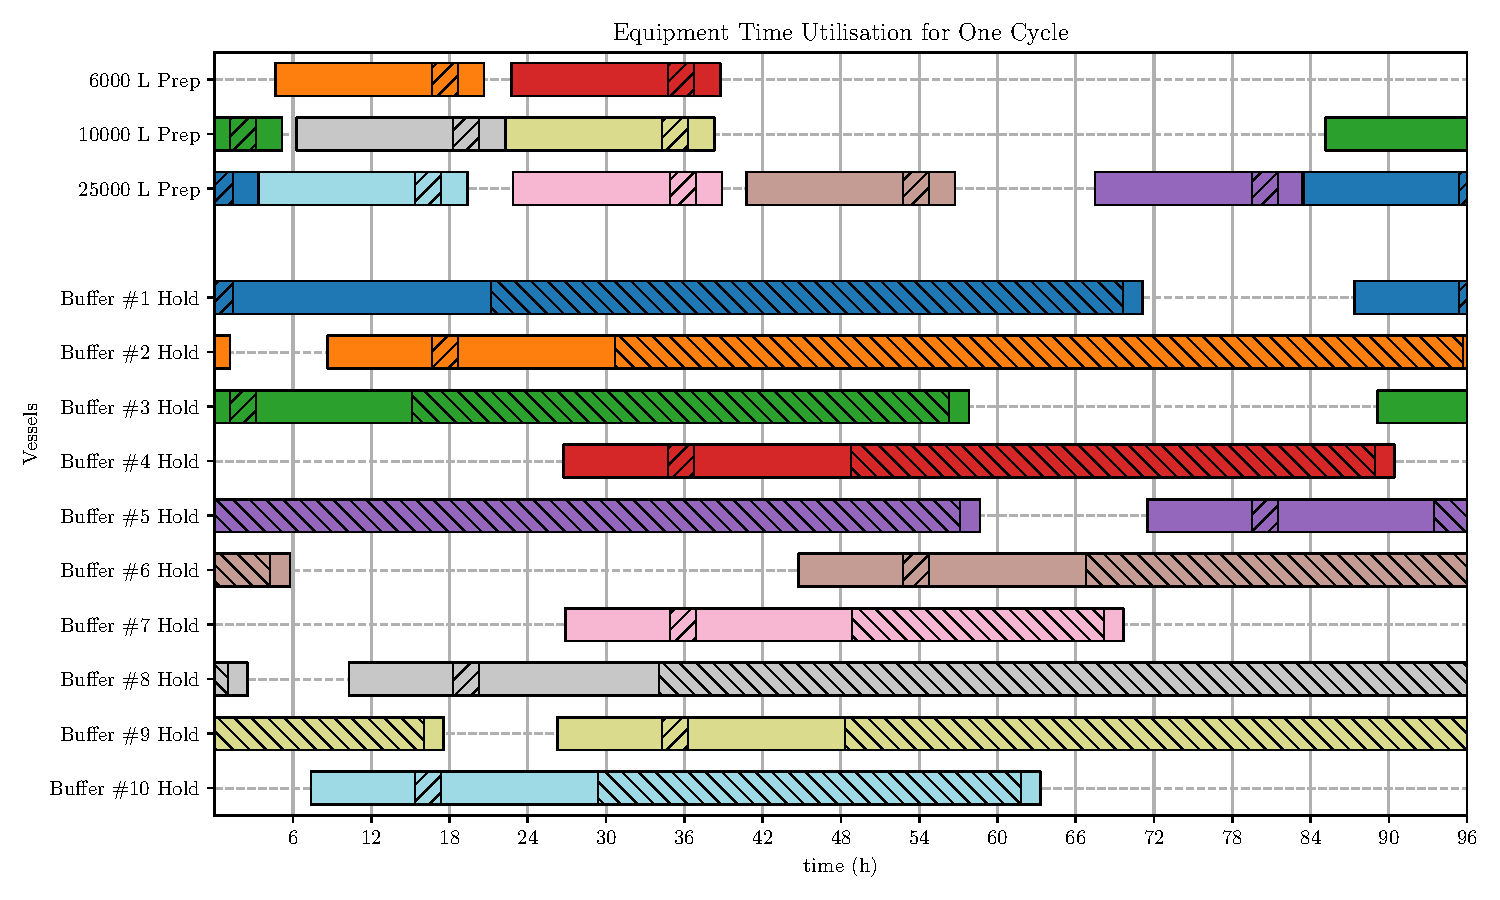
\includegraphics[angle=0,scale=0.55]{../examples/large-scale/plot2.pdf}
    \caption{Equipment Time Utilisation for Large-Scale Example}
    \label{fig.etu}
\end{figure}
